\documentclass[14pt]{extbook}
\usepackage{multicol, enumerate, enumitem, hyperref, color, soul, setspace, parskip, fancyhdr} %General Packages
\usepackage{amssymb, amsthm, amsmath, bbm, latexsym, units, mathtools} %Math Packages
\everymath{\displaystyle} %All math in Display Style
% Packages with additional options
\usepackage[headsep=0.5cm,headheight=12pt, left=1 in,right= 1 in,top= 1 in,bottom= 1 in]{geometry}
\usepackage[usenames,dvipsnames]{xcolor}
\usepackage{dashrule}  % Package to use the command below to create lines between items
\newcommand{\litem}[1]{\item#1\hspace*{-1cm}\rule{\textwidth}{0.4pt}}
\pagestyle{fancy}
\lhead{Module12L}
\chead{}
\rhead{Version B}
\lfoot{9732-2394}
\cfoot{}
\rfoot{Fall 2020}
\begin{document}

\begin{enumerate}
\litem{
Determine the horizontal and/or oblique asymptotes in the rational function below.\[ f(x) = \frac{6x^{3} -23 x^{2} -10 x + 75}{3x^{2} +17 x + 20} \]\begin{enumerate}[label=\Alph*.]
\item \( \text{Oblique Asymptote of } y = 2x -19. \)
\item \( \text{Horizontal Asymptote of } y = -4.0 \text{ and Oblique Asymptote of } y = 2x -19 \)
\item \( \text{Horizontal Asymptote at } y = -4.0 \)
\item \( \text{Horizontal Asymptote of } y = 2.0 \text{ and Oblique Asymptote of } y = 2x -19 \)
\item \( \text{Horizontal Asymptote of } y = 2.0  \)

\end{enumerate} }
\litem{
Determine the horizontal and/or oblique asymptotes in the rational function below.\[ f(x) = \frac{16x^{3} -40 x^{2} -39 x + 45}{4x^{2} +21 x + 20} \]\begin{enumerate}[label=\Alph*.]
\item \( \text{Horizontal Asymptote of } y = 4.0 \text{ and Oblique Asymptote of } y = 4x -31 \)
\item \( \text{Horizontal Asymptote of } y = 4.0  \)
\item \( \text{Horizontal Asymptote of } y = -4.0 \text{ and Oblique Asymptote of } y = 4x -31 \)
\item \( \text{Horizontal Asymptote at } y = -4.0 \)
\item \( \text{Oblique Asymptote of } y = 4x -31. \)

\end{enumerate} }
\litem{
Which of the following functions \textit{could} be the graph below?
\begin{center}
    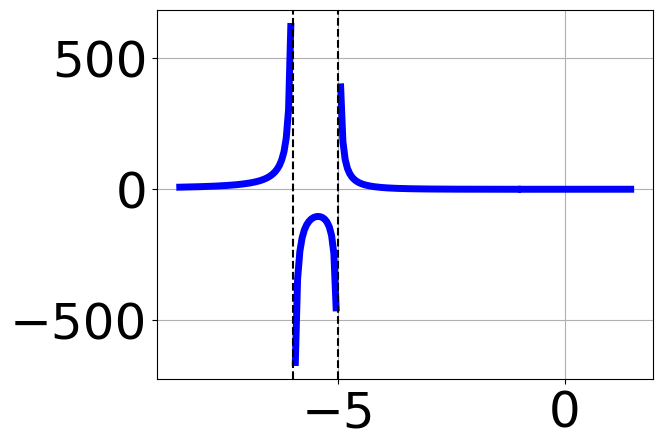
\includegraphics[width=0.5\textwidth]{../Figures/identifyGraphOfRationalFunctionB.png}
\end{center}
\begin{enumerate}[label=\Alph*.]
\item \( f(x)=\frac{x^{3} +2 x^{2} -15 x -36}{x^{3} +4 x^{2} -7 x -10} \)
\item \( f(x)=\frac{x^{3} -6 x^{2} -x + 30}{x^{3} -4 x^{2} -7 x + 10} \)
\item \( f(x)=\frac{x^{3} +6 x^{2} -x -30}{x^{3} +4 x^{2} -7 x -10} \)
\item \( f(x)=\frac{x^{3} -6 x^{2} -x + 30}{x^{3} -4 x^{2} -7 x + 10} \)
\item \( \text{None of the above are possible equations for the graph.} \)

\end{enumerate} }
\litem{
Determine the vertical asymptotes and holes in the rational function below.\[ f(x) = \frac{12x^{3} +37 x^{2} -17 x -60}{6x^{2} +17 x + 12} \]\begin{enumerate}[label=\Alph*.]
\item \( \text{Vertical Asymptotes of } x = -1.5 \text{ and } x = -1.333 \text{ with no holes.} \)
\item \( \text{Holes at } x = -1.5 \text{ and } x = -1.333 \text{ with no vertical asymptotes.} \)
\item \( \text{Vertical Asymptote of } x = 2.0 \text{ and hole at } x = -1.333 \)
\item \( \text{Vertical Asymptotes of } x = -1.5 \text{ and } x = 1.25 \text{ with a hole at } x = -1.333 \)
\item \( \text{Vertical Asymptote of } x = -1.5 \text{ and hole at } x = -1.333 \)

\end{enumerate} }
\litem{
Determine the horizontal and/or oblique asymptotes in the rational function below.\[ f(x) = \frac{-12x^{3} +31 x^{2} -18 x -45}{9x^{3} -36 x^{2} +17 x + 30} \]\begin{enumerate}[label=\Alph*.]
\item \( \text{Vertical Asymptote of } y = -0.750  \)
\item \( \text{None of the above} \)
\item \( \text{Horizontal Asymptote of } y = 0  \)
\item \( \text{Vertical Asymptote of } y = 3  \)
\item \( \text{Horizontal Asymptote of } y = -0.750  \)

\end{enumerate} }
\litem{
Determine the vertical asymptotes and holes in the rational function below.\[ f(x) = \frac{16x^{3} -64 x^{2} +79 x -30}{8x^{2} -22 x + 15} \]\begin{enumerate}[label=\Alph*.]
\item \( \text{Vertical Asymptotes of } x = 1.5 \text{ and } x = 0.75 \text{ with a hole at } x = 1.25 \)
\item \( \text{Vertical Asymptote of } x = 1.5 \text{ and hole at } x = 1.25 \)
\item \( \text{Vertical Asymptotes of } x = 1.5 \text{ and } x = 1.25 \text{ with no holes.} \)
\item \( \text{Holes at } x = 1.5 \text{ and } x = 1.25 \text{ with no vertical asymptotes.} \)
\item \( \text{Vertical Asymptote of } x = 2.0 \text{ and hole at } x = 1.25 \)

\end{enumerate} }
\litem{
Determine the horizontal and/or oblique asymptotes in the rational function below.\[ f(x) = \frac{2x^{2} +3 x -20}{8x^{3} +6 x^{2} -45 x -50} \]\begin{enumerate}[label=\Alph*.]
\item \( \text{Horizontal Asymptote of } y = 4.000 \text{ and Oblique Asymptote of } y = 4x -3 \)
\item \( \text{Horizontal Asymptote of } y = 4.000  \)
\item \( \text{Horizontal Asymptote at } y = -4.000 \)
\item \( \text{Oblique Asymptote of } y = 4x -3. \)
\item \( \text{Horizontal Asymptote of } y = 0 \)

\end{enumerate} }
\litem{
Which of the following functions \textit{could} be the graph below?
\begin{center}
    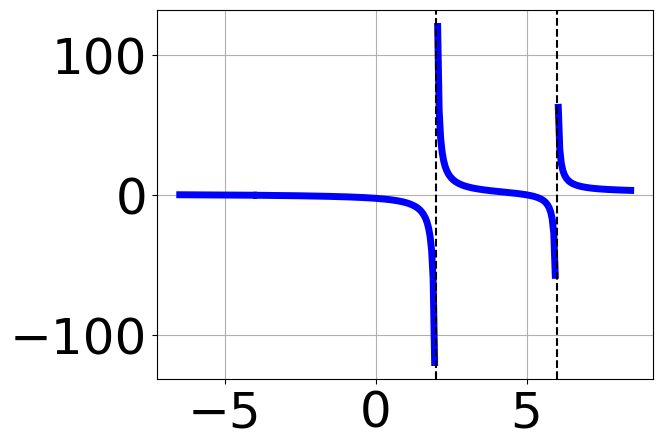
\includegraphics[width=0.5\textwidth]{../Figures/identifyGraphOfRationalFunctionCopyB.png}
\end{center}
\begin{enumerate}[label=\Alph*.]
\item \( f(x)=\frac{x^{3} -4 x^{2} -9 x + 36}{x^{3} +7 x^{2} +4 x -12} \)
\item \( f(x)=\frac{x^{3} -1 x^{2} -26 x -24}{x^{3} -7 x^{2} +4 x + 12} \)
\item \( f(x)=\frac{x^{3} + x^{2} -26 x + 24}{x^{3} +7 x^{2} +4 x -12} \)
\item \( f(x)=\frac{x^{3} -1 x^{2} -26 x -24}{x^{3} -7 x^{2} +4 x + 12} \)
\item \( \text{None of the above are possible equations for the graph.} \)

\end{enumerate} }
\litem{
Determine the vertical asymptotes and holes in the rational function below.\[ f(x) = \frac{6x^{3} +23 x^{2} +9 x -18}{4x^{2} -4 x -15} \]\begin{enumerate}[label=\Alph*.]
\item \( \text{Vertical Asymptote of } x = 2.5 \text{ and hole at } x = -1.5 \)
\item \( \text{Vertical Asymptotes of } x = 2.5 \text{ and } x = -1.5 \text{ with no holes.} \)
\item \( \text{Vertical Asymptotes of } x = 2.5 \text{ and } x = 0.667 \text{ with a hole at } x = -1.5 \)
\item \( \text{Holes at } x = 2.5 \text{ and } x = -1.5 \text{ with no vertical asymptotes.} \)
\item \( \text{Vertical Asymptote of } x = 1.5 \text{ and hole at } x = -1.5 \)

\end{enumerate} }
\litem{
Determine the vertical asymptotes and holes in the rational function below.\[ f(x) = \frac{12x^{3} +73 x^{2} +112 x + 48}{6x^{2} +17 x + 12} \]\begin{enumerate}[label=\Alph*.]
\item \( \text{Vertical Asymptote of } x = 2.0 \text{ and hole at } x = -1.333 \)
\item \( \text{Holes at } x = -1.5 \text{ and } x = -1.333 \text{ with no vertical asymptotes.} \)
\item \( \text{Vertical Asymptotes of } x = -1.5 \text{ and } x = -1.333 \text{ with no holes.} \)
\item \( \text{Vertical Asymptote of } x = -1.5 \text{ and hole at } x = -1.333 \)
\item \( \text{Vertical Asymptotes of } x = -1.5 \text{ and } x = -0.75 \text{ with a hole at } x = -1.333 \)

\end{enumerate} }
\end{enumerate}

\end{document}